\subsection{Abläufe modellieren}
\label{sec:Kap-6.3.2}

Die im vorherigen Kapitel~\ref{sec:Kap-6.3.1} behandelten Anwendungsfalldiagramme modellieren die Interaktionen der Nutzer mit dem System. Sie beschreiben damit zwar, welche Anwendungsfälle das System gewährleisten können muss. Dabei blenden sie aber aus, wie diese Interaktionen genau ablaufen, da sie weder Reihenfolgen von Interaktionen berücksichtigen, noch modellieren, was während der Interaktion im System geschieht. Über Aktivitätsdiagramme lässt sich dies darstellen.

Aktivitätsdiagramme modellieren Abläufe, wobei es sich zum Beispiel um Geschäftsprozesse oder die Abläufe von Anwendungsfällen, aber ebenso auch um Algorithmen handeln kann. Man kann Aktivitätsdiagramme in unterschiedlichen Abstraktionsgraden und für unterschiedliche Zwecke in allen Kernprozessen des Softwareengineering einsetzen. Sie sind extrem mächtig, da sie sehr viele unterschiedliche Notationselemente zur Verfügung stellen. Da Aktivitätsdiagramme auf der Semantik von Petrinetzen basieren, lassen sich mit ihnen sogar parallele Abläufe modellieren.

% Abbildung Leserführung
\sttpAbbildungskasten{Bilder/Kapitel-6/UML-Diagramme-Kap-6-Aktivitaetsdiagramm.pdf}{0.7} 

Im Rahmen des Requirements Engineering werden mit Aktivitätsdiagrammen hauptsächlich die Abläufe von Anwendungsfällen oder komplexe Geschäftsprozesse der Domäne modelliert. Beides erfolgt noch stark Nutzersicht-zentriert, so dass in Aktivitätsdiagrammen des Requirements Engineering in der Regel nur ein Bruchteil der zur Verfügung stehenden Notationselemente dieser Diagrammart verwendet wird.

\begin{figure}
	\centering
	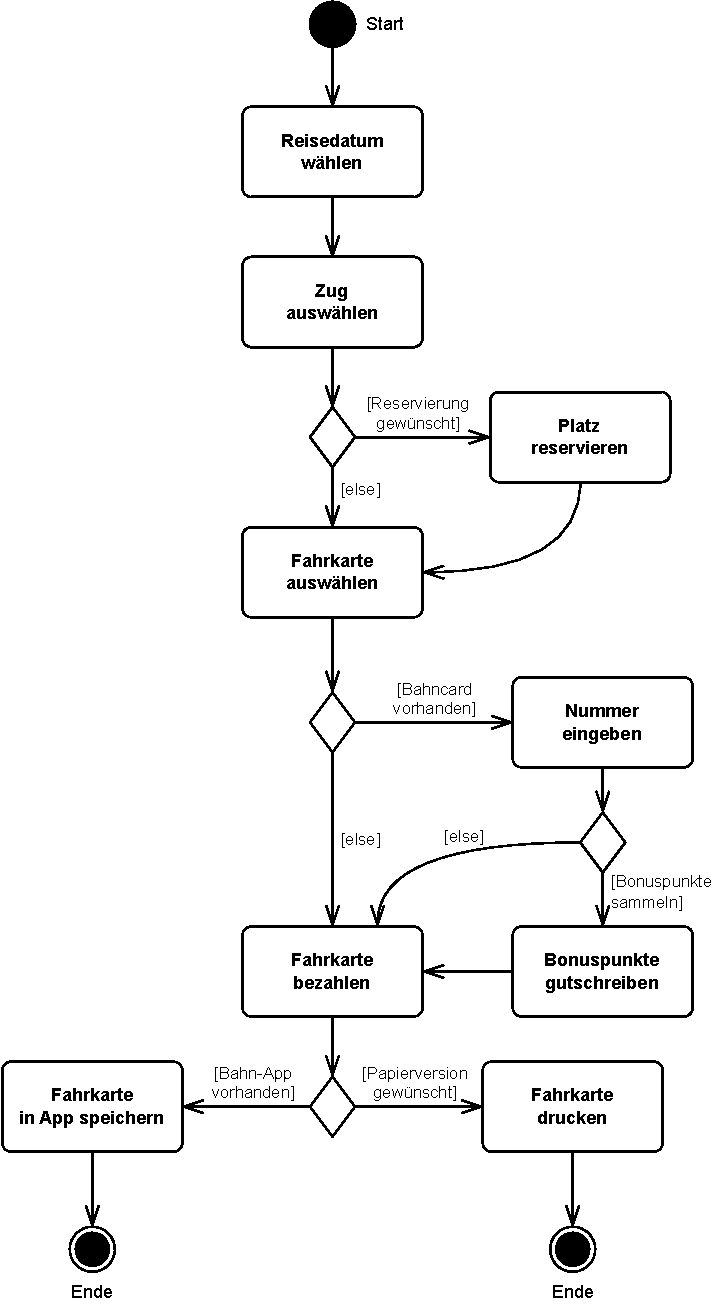
\includegraphics[width=0.8\textwidth]{Bilder/Kapitel-6/aktivitaetsdiagramm_fahrkarte_kaufen.pdf}
	\caption{Aktivitätsdiagramm für die Aktivität Fahrkartenkauf}
	\label{fig:aktivitaetsdiagramm_fahrkarte_kaufen}
\end{figure}

Abbildung~\ref{fig:aktivitaetsdiagramm_fahrkarte_kaufen} zeigt ein Aktivitätsdiagramm für die Aktivität Fahrkartenkauf. Mit den abgerundeten Rechtecken werden die einzelnen \textit{Aktionen} des Fahrkartenkaufs dargestellt. Die Pfeile repräsentieren den \textit{Kontrollfluss}, die Ausführungsreihenfolge zwischen den Aktionen. Der schwarz ausgemalte Kreis ist der \textit{Startknoten}, der spezifiziert, bei welcher Aktion die Aktivität beginnt. Die Rauten sind so genannte \textit{Entscheidungsknoten}. Ein Entscheidungsknoten hat genau einen eingehenden Kontrollfluss und beliebig viele ausgehende, von denen bei einer konkreten Ausführung der Aktivität (einem Ablauf) aber nur genau einer fortgeführt wird. (Man kann auch parallele Kontrollflüsse modellieren, aber die dafür nötigen Elemente haben wir in diesem Diagramm nicht verwendet.) Die ausgehenden Pfeile des Entscheidungsknotens sind mit Bedingungen (engl. guard), die in eckigen Klammern notiert werden, versehen. Die \textit{Guards} eines Entscheidungsknotens müssen disjunkt sein und alle Auswahlmöglichkeiten abdecken, so dass der weitere Kontrollfluss eindeutig festgelegt ist. Ein oder mehrere \textit{Endknoten} (schwarzer Kreis mit weißer Umrandung) spezifizieren, nach welchen Aktionen eine Aktivität enden kann.

Analog zum Element Entscheidungsknoten bietet das Aktivitätsdiagramm auch einen \textit{Verbindungsknoten} an, wenn Kontrollflüsse wieder zusammenlaufen. Dieser wird ebenfalls über eine Raute dargestellt. Er unterscheidet sich vom Entscheidungsknoten dadurch, dass beliebig viele Kontrollflüsse hereinführen, aber nur genau einer herausführt. Häufig lässt man Verbindungsknoten im Diagramm weg und führt die Kontrollflüsse direkt in der Aktion wieder zusammen: In Abbildung \ref{fig:aktivitaetsdiagramm_fahrkarte_kaufen} hat die Aktion \sttpUMLText{Fahrkarte auswählen} zwei eingehende Pfeile, einen ausgehend von der Aktion \sttpUMLText{Platz} \sttpUMLText{reservieren} und einen ausgehend vom Entscheidungsknoten hinter \sttpUMLText{Zug auswählen}. Bei Verwendung eines Verbindungsknotens würden diese beiden Pfeile in einen Verbindungsknoten führen und aus diesem Verbindungsknoten dann ein Pfeil zu \sttpUMLText{Fahrkarte} \sttpUMLText{auswählen}. Die UML erlaubt es, auch auf Entscheidungsknoten zu verzichten, aber das macht ein Aktivitätsdiagramm meistens unübersichtlicher. Zumindest bei Aktivitätsdiagrammen im Requirements Engineering sollte man Entscheidungsknoten daher nicht weglassen.

\begin{figure}[h!]
	\centering
	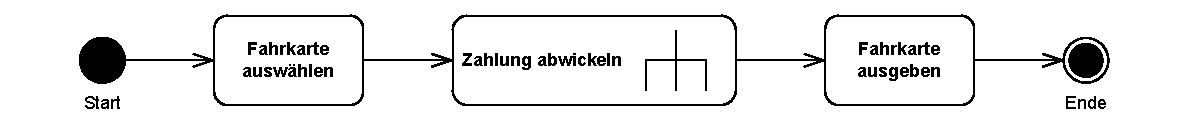
\includegraphics[width=\textwidth]{Bilder/Kapitel-6/aktivitaetsaufruf_zahlung.pdf}
	\caption{Aktivitätsaufruf Zahlung abwickeln}
	\label{fig:aktivitaetsaufruf_zahlung}
\end{figure}

\begin{figure}[h!]
	\centering
	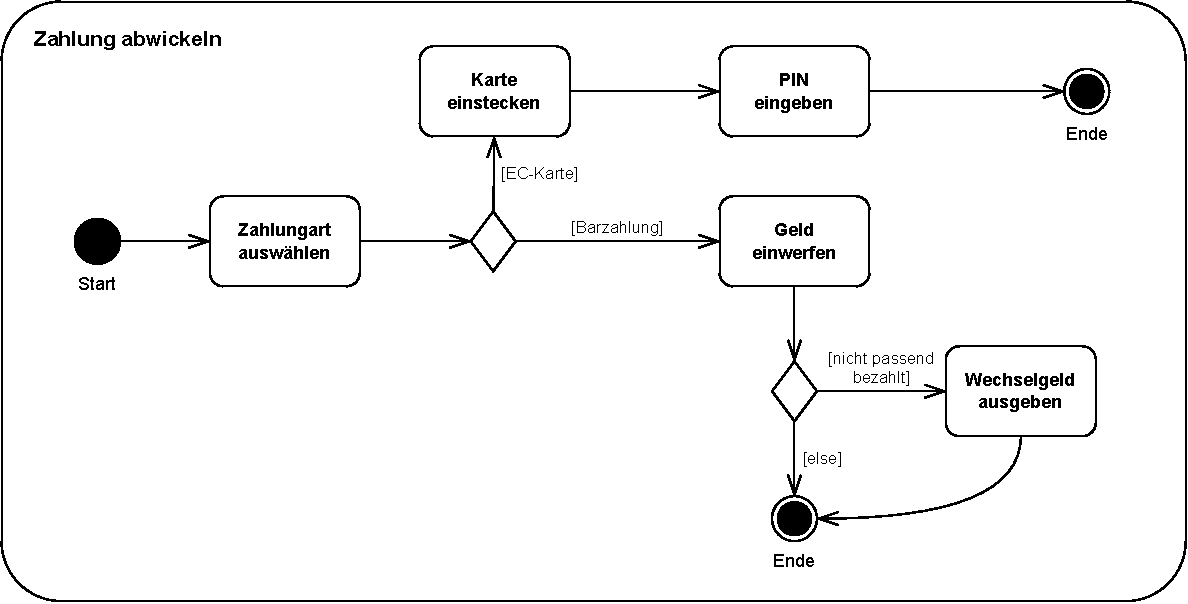
\includegraphics[width=\textwidth]{Bilder/Kapitel-6/aktivitaetsdiagramm_zahlung_abwickeln.pdf}
	\caption{Aktivitätsdiagramm Zahlung abwickeln}
	\label{fig:aktivitaetsdiagramm_zahlung_abwickeln}
\end{figure}

Wenn Aktivitäten sehr kleinschrittig (viele einzelne Aktionen) beschrieben werden sollen, können Aktivitätsdiagramme schnell unübersichtlich werden. Oft bietet es sich an, ein Aktivitätsdiagramm auf einem hohen Abstraktionsniveau als Übersicht zu haben und dessen einzelne Aktionen in jeweils eigenen Diagrammen verfeinert zu modellieren. Abbildung~\ref{fig:aktivitaetsaufruf_zahlung} zeigt ein sehr übersichtliches Diagramm für eine Aktivität Fahrkarte kaufen an einem Automaten. Bei der Aktion Zahlung abwickeln in diesem Diagramm ist durch das „Gabel“-Symbol rechts im Kästchen gekennzeichnet, dass hier ein Aktivitätsaufruf erfolgt. Und zwar der Aufruf der Aktivität Zahlung abwickeln, die in einem eigenen Aktivitätsdiagramm modelliert ist. Dieses ist in Abbildung~\ref{fig:aktivitaetsdiagramm_zahlung_abwickeln} dargestellt. 


\minisec{Aktivitätsdiagramme im Rahmen der Domänenmodellierung}

In Rahmen der Domänenmodellierung werden Aktivitätsdiagramme vor allem zur Modellierung von Geschäftsprozessen der Domäne eingesetzt. Häufig geht es dabei auch darum, herauszufinden, welche Akteure in welcher Art und Weise am Geschäftsprozess beteiligt sind, also wer welche Tätigkeiten im Rahmen des Geschäftsprozesses ausführt. Das UML-Aktivitätsdiagramm bietet das Element Aktivitätsbereich an, um die Verantwortung für Aktionen bestimmten Akteuren zuzuordnen. Für diejenigen, die BPMN (Business Process Model and Notation, eine eigene Modellierungssprache für Geschäftsprozesse) kennen: Aktivitätsbereiche, die man auch noch schachteln und gruppieren kann, sind ein ähnliches Prinzip wie Pools und Lanes in BPMN. 

\begin{figure}[h!]
	\centering
	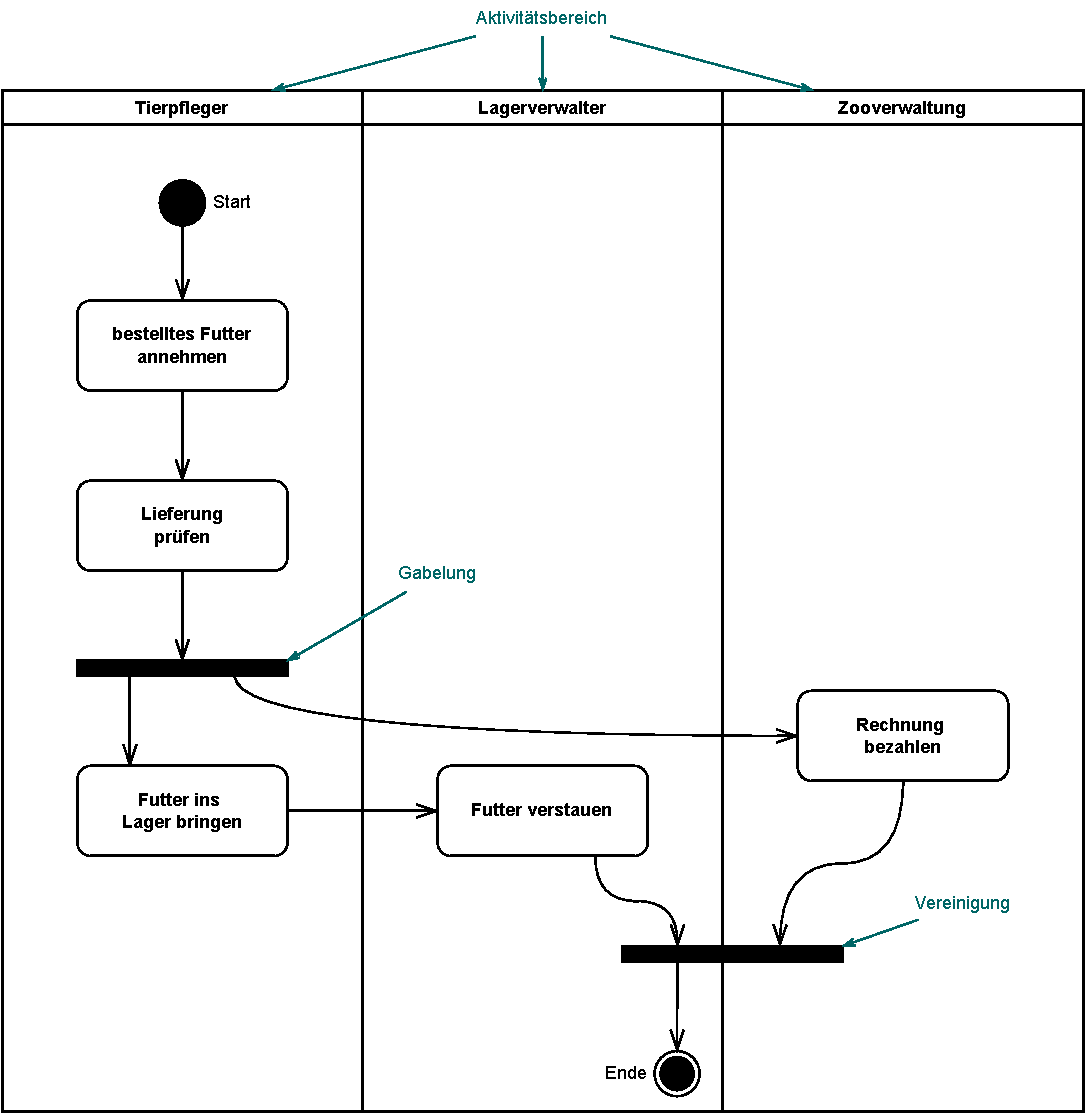
\includegraphics[width=\textwidth]{Bilder/Kapitel-6/aktivitaetsdiagramm_futterannahme.pdf}
	\caption{Aktivitätsdiagramm Futterannahme}
	\label{fig:aktivitaetsdiagramm_futterannahme}
\end{figure}

Abbildung~\ref{fig:aktivitaetsdiagramm_futterannahme} zeigt ein Diagramm mit drei Aktivitätsbereichen für die Akteure \linebreak
\sttpUMLText{Tierpfleger}, \sttpUMLText{Lagerverwalter} und \sttpUMLText{Zooverwaltung} für eine Aktivität Futterannahme. Durch die Platzierung in den Aktivitätsbereichen ist deutlich, wer welche Aktionen ausführt. Die Abbildung zeigt außer den Aktivitätsbereichen auch die Elemente für die Modellierung paralleler Kontrollflüsse (schwarze Balken). 

Diese sind unabhängig von den Aktivitätsbereichen, hätten also auch in den vorherigen Diagrammen verwendet werden können. Der schwarze Balken im Aktivitätsbereich des Tierpflegers ist eine so genannte \textit{Gabelung}. Die Gabelung teilt einen Kontrollfluss in mehrere parallele Kontrollflüsse auf. Das Pendant, um die Parallelität wieder zu beenden, ist die so genannte \textit{Vereinigung}, die Sie rechts unten im Diagramm sehen. Die Vereinigung fasst mehrere Kontrollflüsse zu einem Kontrollfluss zusammen. Hier in der Abbildung modelliert sie, dass sowohl die Aktion \sttpUMLText{Futter verstauen} vom Akteur \sttpUMLText{Lagerverwalter} als auch die Aktion \sttpUMLText{Rechnung bezahlen} vom Akteur \sttpUMLText{Zooverwaltung} abgeschlossen sein müssen, bevor die Aktivität Futterannahme beendet ist.


